\documentclass[10pt,a4paper]{article}
\usepackage[utf8]{inputenc}
\usepackage{amsmath}
\usepackage{gensymb}
\usepackage{amsfonts}
\usepackage{siunitx}
\usepackage[european]{circuitikz}
\usepackage{geometry}
\newgeometry{tmargin=2cm, bmargin=2cm, lmargin=2cm, rmargin=2cm}
\usepackage{amssymb}
\usepackage{polski}
\usepackage{graphicx}
\author{\textbf{T. Fąs}}
\title{\textbf{PRZEWODNICTWO CIEPLNE MIEDZI}}
\begin{document}
\maketitle

\begin{center}
\textbf{\subsection*{STRESZCZENIE}}
\end{center}
Celem doświadczenia było wyznaczenie współczynnika $\lambda$ przewodnictwa cieplnego miedzi. Wartość otrzymana w eksperymencie wynosi $\lambda=(344\pm12)$ W/mK, która w porównaniu z wartościami tablicowymi nie przechodzi testu 3$\sigma$.
\begin{center}
\textbf{\subsection*{WSTĘP}}
\end{center}
Jeśli między badanymi ciałami istnieje różnica temperatur, to zgodnie z prawami termodynamiki będzie istniał przepływ ciepła z ciała cieplejszego do zimniejszego. Z tym przepływem związany jest współczynnik $\lambda$ przewodnictwa cieplnego. Jest on miarą zdolności ciała do transportu energii. Im większy współczynnik, tym więcej energii jest w stanie przepłynąć przez to ciało. Ilość przepływu ciepła $Q$ w czasie dla ciała, którego dwa różne punkty $x$ mają różną temperaturę $T$, jest opisana przez prawo Fouriera:
\begin{equation}
\dfrac{dQ}{dt}=-\lambda S \dfrac{\partial T}{\partial x},
\end{equation}
gdzie $S$ jest przekrojem poprzecznym ciała. Równanie (1) jest słuszne tylko dla stałej różnicy temperatur, czyli $\partial T/\partial x=const$. Jeśli tak, to ${dQ}/{dt}$ również jest wartością stałą. Tak więc, żeby wyznaczyć współczynnik $\lambda$ z Równania (1) należy badać ciało w stanie stacjonarnym.

\begin{center}
\textbf{\subsection*{UKŁAD DOŚWIADCZALNY}}
\end{center}
Układ składał się z pręta miedzianego o średnicy $D=(6\pm0,1)$ mm umieszczonego w izolowanej obudowie, którego jeden koniec był zanurzony w wodzie, a drugi koniec był podłączony do grzałki. W różnych miejscach pręta zostały zamocowane termopary miedź-konstantan, które pozwoliły na zmierzenie napięcia między złączem najbliższym grzałce, a każdym kolejnym, a co za tym idzie, różnicy temperatur. między tymi punktami. Do pomiarów napięcia z termopar wykorzystano mikrowoltomierz NI-9211, który był podłączony do komputera. Wyniki były zapisywane w pamięci komputera. Warto dodać, że minimalna niepewność związana z mikrowoltomierzem wynosi 5 $\mu$V.
 Dodatkowo wykorzystano dwa mierniki CHY 38 do rejestracji napięcia i natężenia związanego z grzałką. Grzałka byłą podłączona do zasilacza o kontrolowanym napięciu, co pozwalało na kontrolę mocy grzałki. 
 
Pomiary były przeprowadzana dla kilku wartości mocy grzałki. Każdy z nich był przeprowadzany tak długo, aż napięcia na termoparach ustabilizowały się. Było to znakiem, że ustaliła się stałą różnica temperatur między danymi punktami.
\begin{center}
\textbf{\subsection*{WYNIKI POMIARÓW}}
\end{center}
Pomiary przeprowadzono dla pięciu rożnych wartości napięcia na grzałce. Wartości te przedstawiono w Tabeli 1. Na samym początku wykonano też jeden pomiar bez grzania. Ilość punktów pomiarowych związana z tymi pomiarami jest zbyt duża, by umieszczać je w raporcie.
\begin{table}[h!]
\centering
\caption{Napięcia, natężenia i ich niepewności}
\begin{tabular}{|c|c|c|c|c|c|}
\hline
Pomiar           & 1      & 2      & 3      & 4      & 5      \\ \hline
Napięcie $U$ [V]   & 6,00   & 7,00   & 8,01   & 9,01   & 10,0   \\ \hline
Natężenie $I$ [A]  & 0,0700 & 0,0817 & 0,0938 & 0,1055 & 0,1177 \\ \hline
Niepewność $U$ [V] & 0,04   & 0,0450 & 0,0500 & 0,0551 & 0,0600 \\ \hline
Niepewność $I$ [A] & 0,0008 & 0,0009 & 0,0010 & 0,0012 & 0,0013 \\ \hline
\end{tabular}
\end{table}
\begin{center}
\textbf{\subsection*{ANALIZA DANYCH}}
\end{center}
W pierwszej kolejności wykonano wykres związany z napięciami przy wyłączonej grzałce. Jest on pokazany na Rysunku 1. Wartości napięć są poniżej wartości ich niepewności, a z ich chaotyczności można wnioskować, iż rozkład temperatur na pręcie był w przybliżeniu jednorodny, a wymiana ciepła z otoczeniem jest bliska zeru.

\begin{figure}[h!]
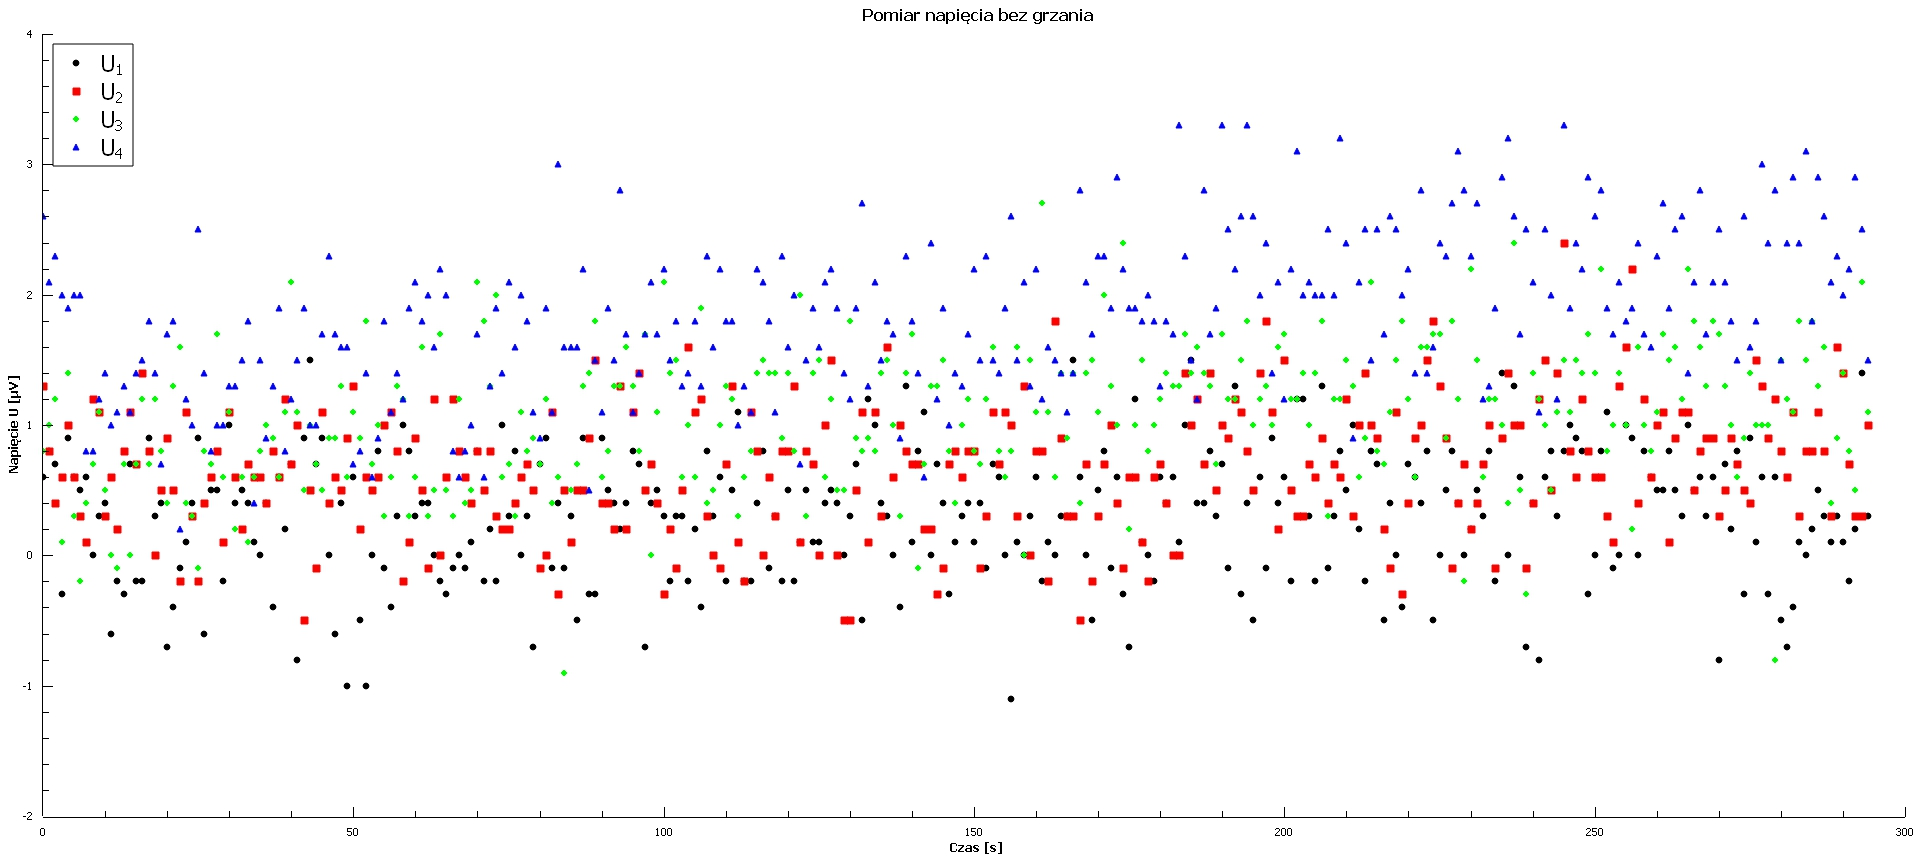
\includegraphics[width=15cm]{rap8rys1} 
\centering
\caption{Napięcia bez grzania}
\end{figure}

Niepewności $u$ związanie z pomiarem napięć $V$ na mikrowoltomierzu obliczono, korzystając ze wzoru:
\begin{equation}
u_{\mu V}=0,001\cdot V+5 \, \mu V,
\end{equation}
Jak już wspomniano wcześniej, niepewność ta nie jest mniejsza od 5 $\mu$V, co jest ważne w przypadku małych wartości napięć. 

Niepewności $u$ dla mierników CHY 38, związanych z pomiarami napięcia $U$ i natężenia $I$ obliczono z następujących wzorów:
\begin{equation}
u_{U}=0,005\cdot U+0,01 \, V
\end{equation}
\begin{equation}
u_{I}=0,01\cdot I+0,0001 \, A
\end{equation}
Wartości niepewności $u_{U}$ i $u_{I}$ zostały umieszczone w Tabeli 1.

Napięcie $V$ na termoparach jest dane funkcją:
\begin{equation}
V(t)=V_{\infty}-V_{0}\exp((t_{0}-t)/\tau)
\end{equation}
gdzie $V_{\infty}$, $V_{0}$, $t_{0}$ i $\tau$ są parametrami dopasowania. Dla bardzo długiego czasu wartość eksponensu dąży do zera, więc dominującym czynnikiem staje się $V_{\infty}$. Jest to szukana wartość napięcia w stanie stacjonarnym. Wartość $V_{\infty}$ jest wprost proporcjonalna do różnicy temperatur związanych punktami pomiaru napięcia. Współczynnik proporcjonalności dla złącza miedź-konstantan wynosi $c=40,9\pm0,2$ $\mu$V/K.

W celu dopasowania krzywej do punktów pomiarowych wykorzystano program SciDAVis. Niepewności pomiarów obliczono z Równania (2) i uwzględniono je w analizie. Wyniki dopasowań dla pomiaru pierwszego przedstawione są na Rysunku (2).
\begin{figure}[h!]
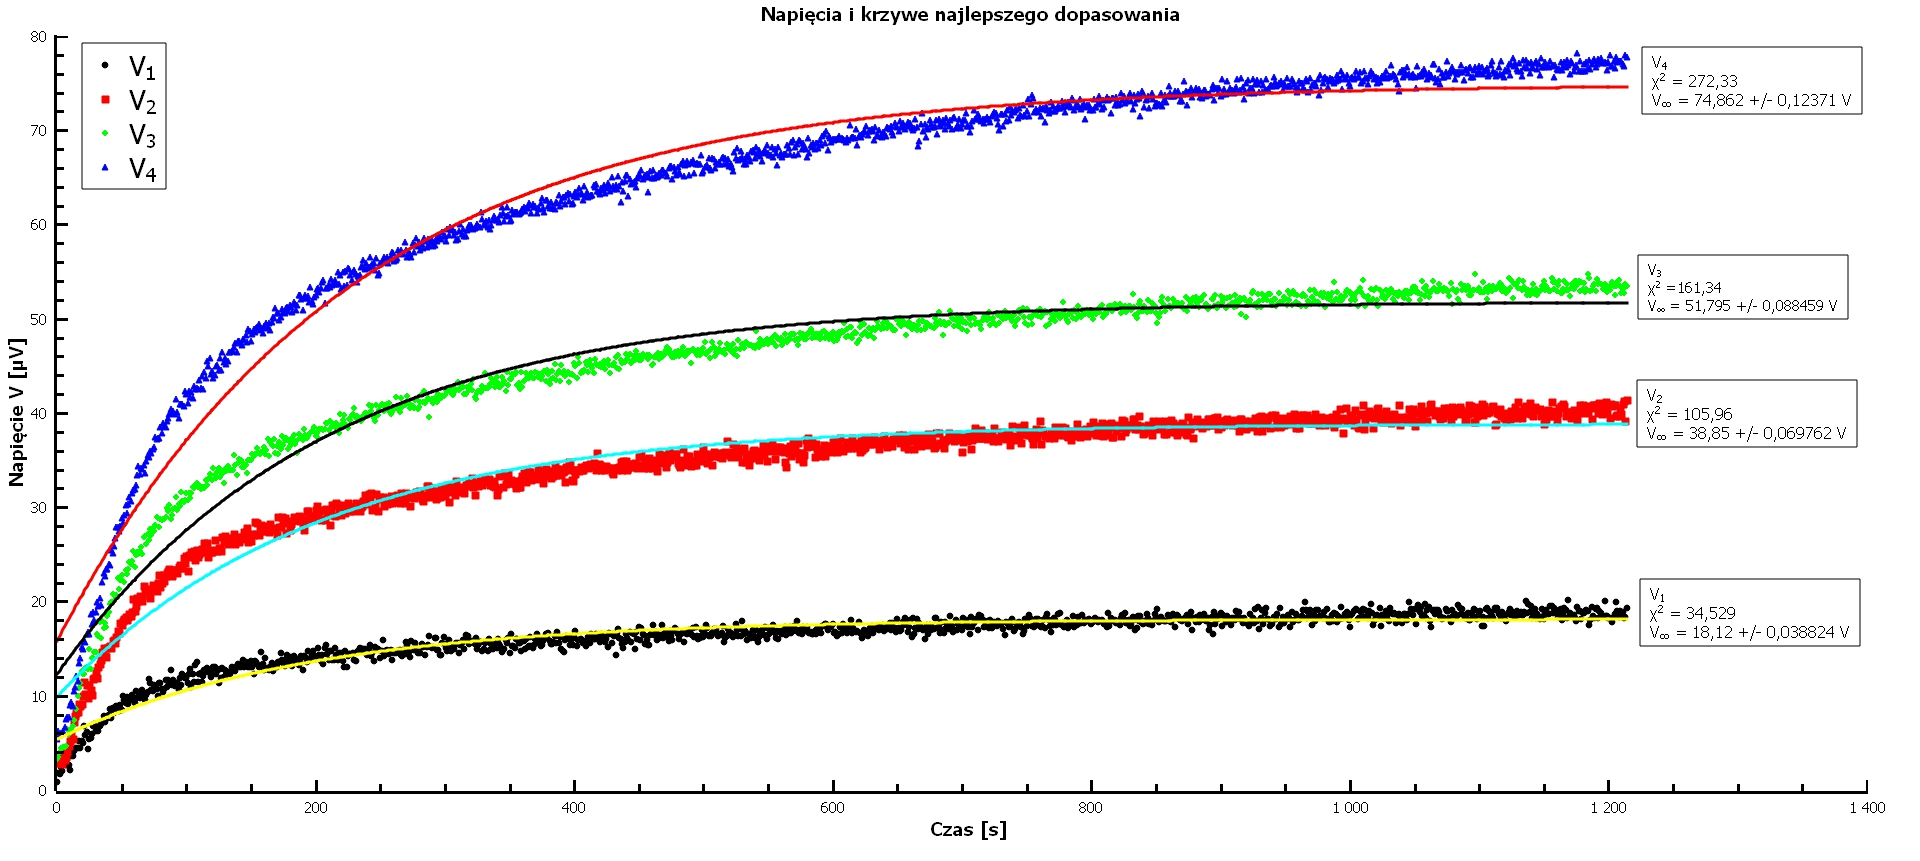
\includegraphics[width=15cm]{rap8rys2} 
\centering
\caption{Dopasowanie krzywej: pomiar 1.}
\end{figure}
W ramkach podano wartości $V_{\infty}$ oraz wartości $\chi^2$ W tym przypadku na wykres składa się ponad tysiąc punktów pomiarowych przy czterech parametrach, co daje wartości krytyczne $\chi^2$ przekraczające 100, np. dla 1000 stopni swobody i dla prawdopodobieństwa $p=0,005$ $\chi_{0}^{2}=1118.95$. Jak widać, krzywe przechodzą test $\chi^2$ pomimo wizualnych odstępstw od punktów pomiarowych. Dzieje się tak, ponieważ niepewności napięcia są znaczne.
 
Analogiczne wykresy dla kolejnych pomiarów są przedstawione na Rysunkach 3-6.

\begin{figure}[h!]
\centering
\begin{minipage}{0.5\textwidth}
  \centering
  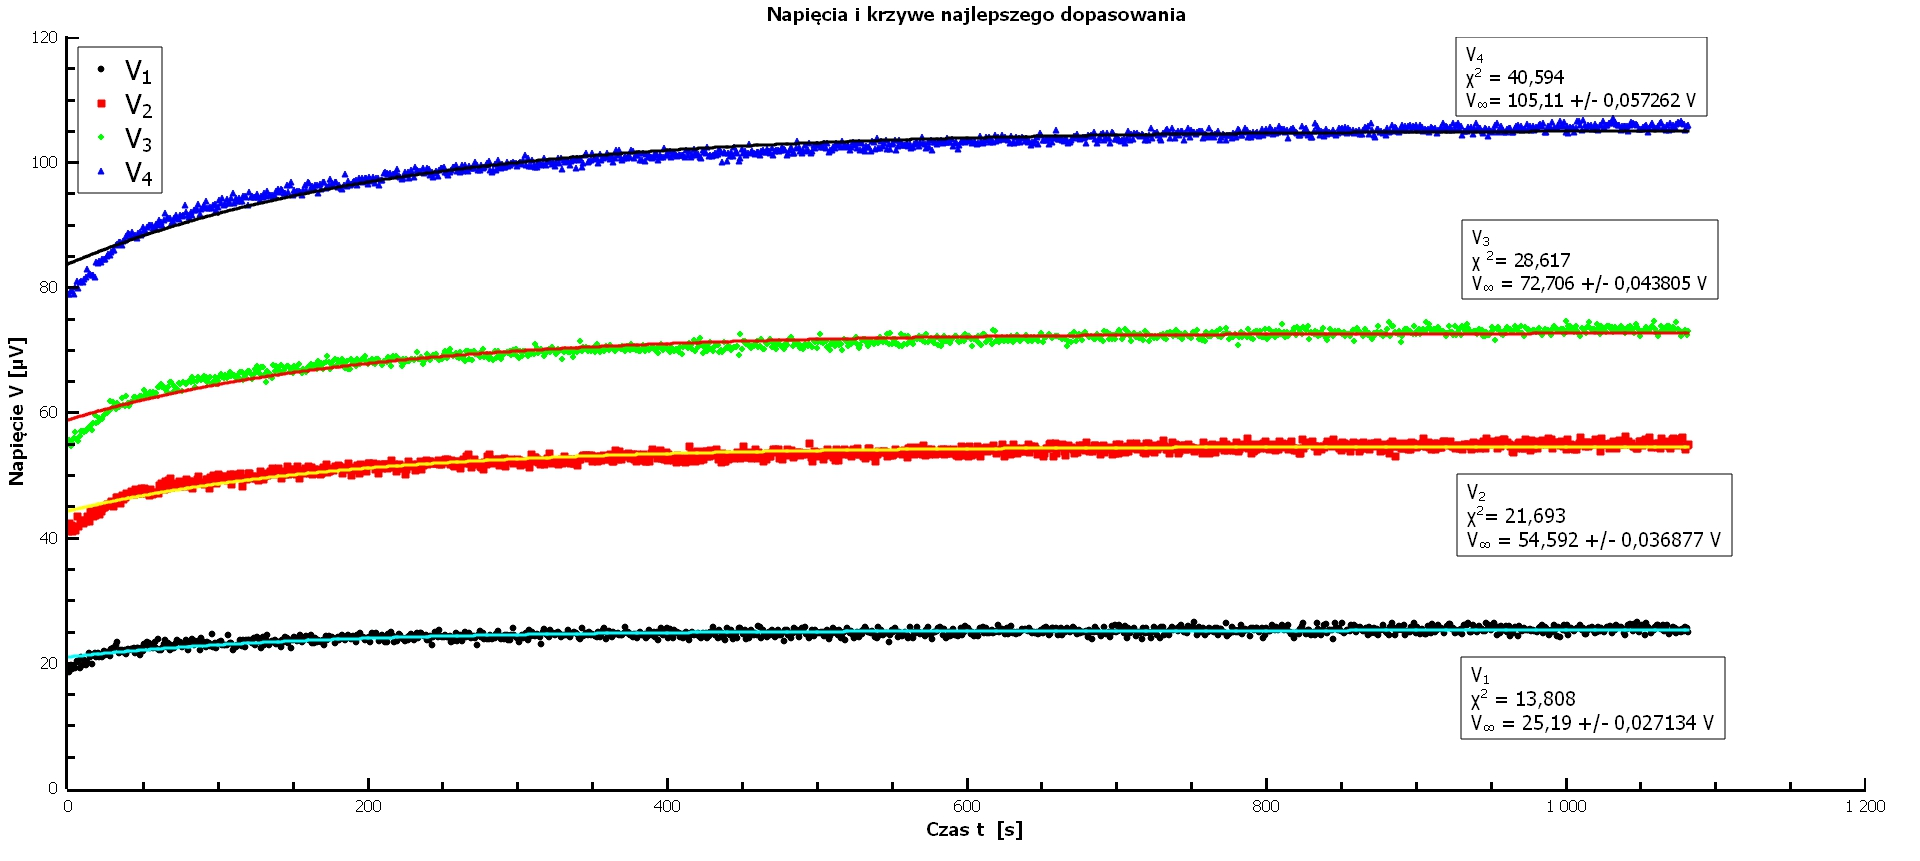
\includegraphics[width=8cm, height=5cm ]{rap8rys3} 
\caption{Dopasowanie krzywej: pomiar 2.}
\end{minipage}%
\begin{minipage}{0.5\textwidth}
  \centering
  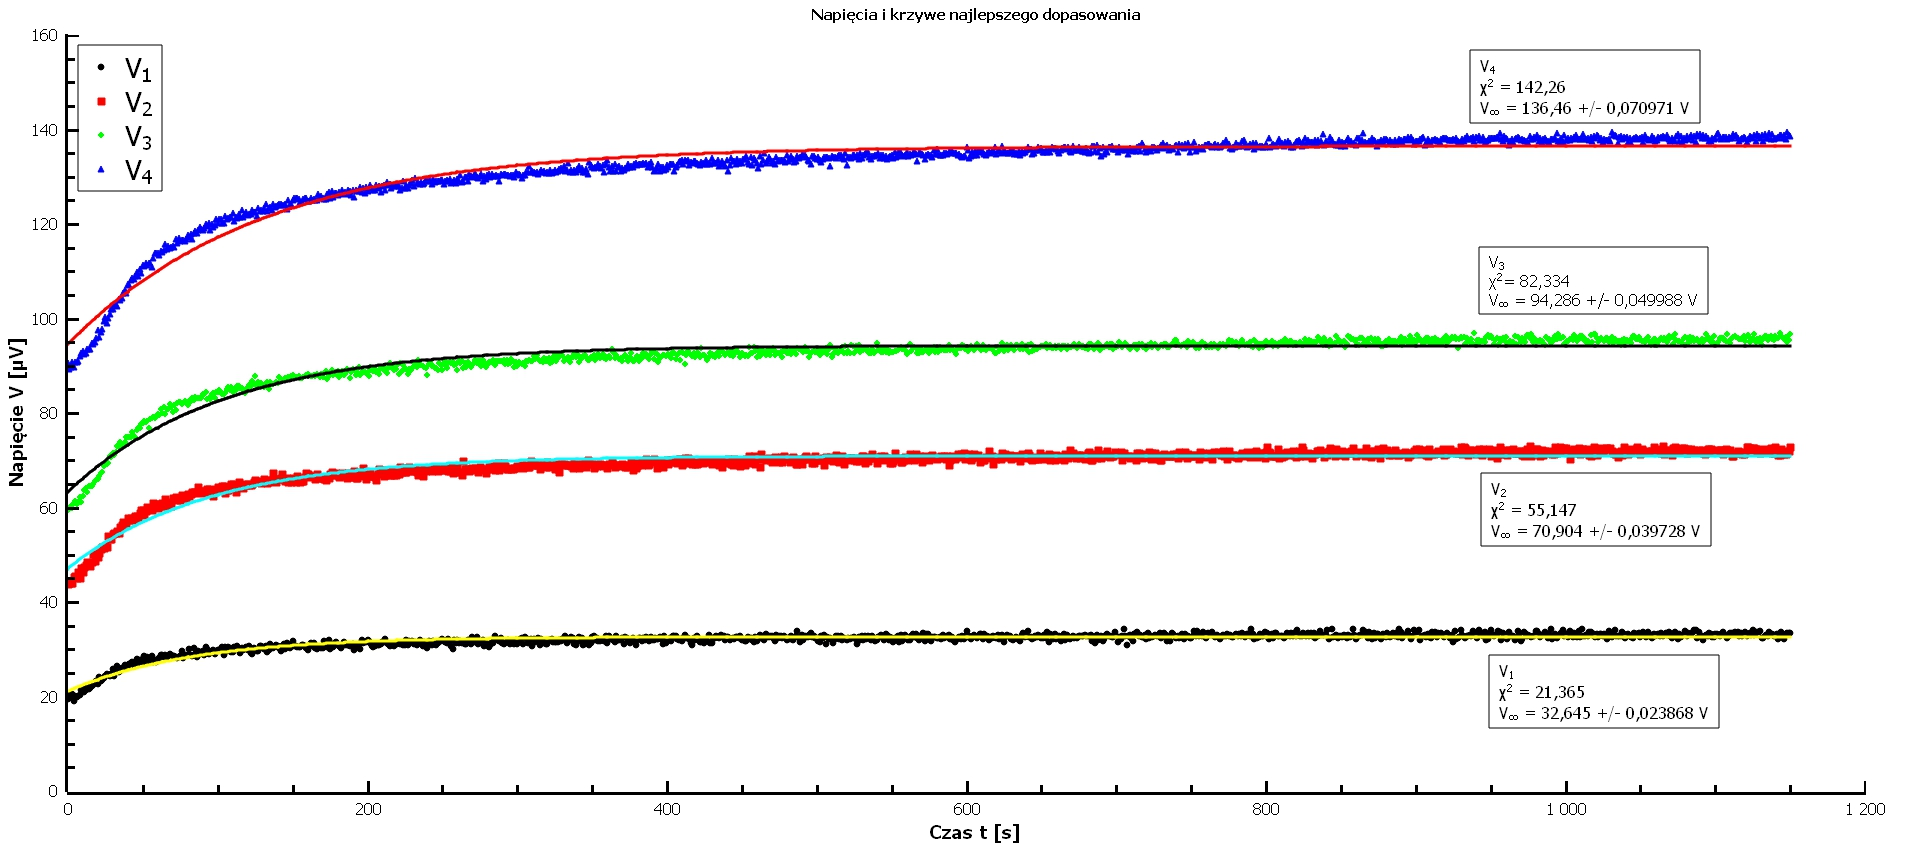
\includegraphics[width=8cm, height=5cm ]{rap8rys4} 
\caption{Dopasowanie krzywej: pomiar 3.}
\end{minipage}
\end{figure}

\begin{figure}[h!]
\centering
\begin{minipage}{0.5\textwidth}
  \centering
  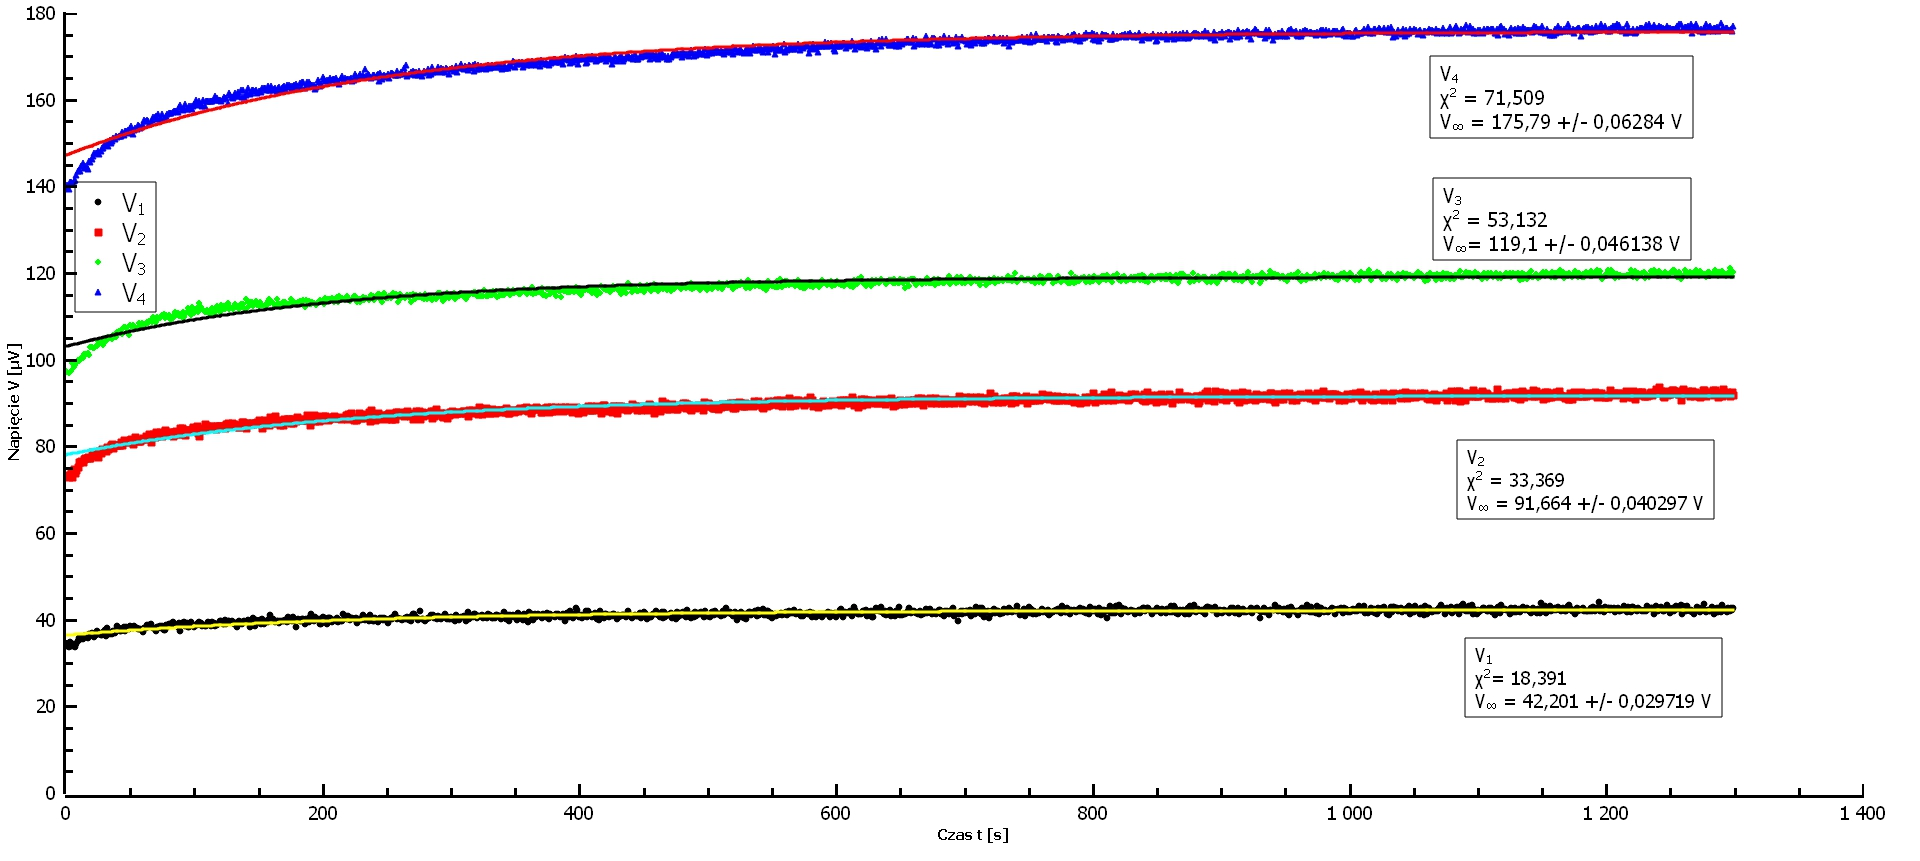
\includegraphics[width=8cm, height=5cm ]{rap8rys5} 
\caption{Dopasowanie krzywej: pomiar 4.}
\end{minipage}%
\begin{minipage}{0.5\textwidth}
  \centering
  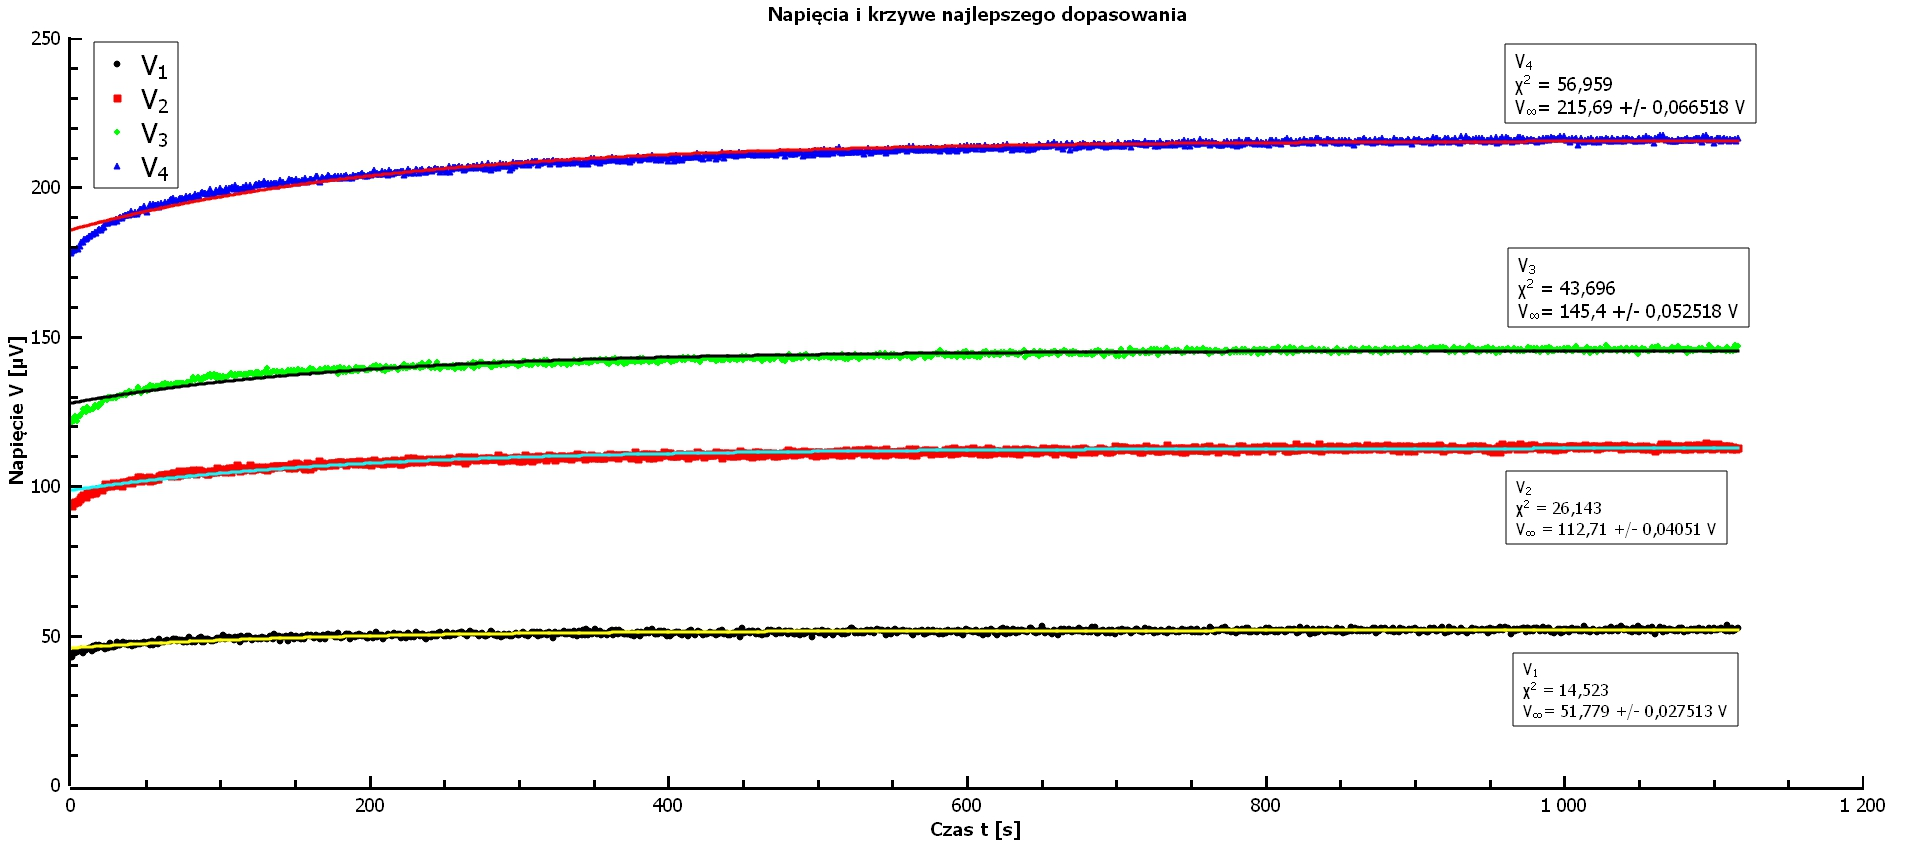
\includegraphics[width=8cm, height=5cm ]{rap8rys6} 
\caption{Dopasowanie krzywej: pomiar 5.}
\end{minipage}
\end{figure}
 

W Tabelach 2-6 zebrano wszystkie współczynniki $V_{\infty}$ wraz z ich niepewnościami. Dodatkowo dopasowano te współczynniki do odpowiednich odległości na pręcie jak i obliczono różnicę temperatur. Niepewność różnic temperatur wyznaczono, korzystając z propagacji małych błędów wyrażającej się wzorem:
 \begin{equation}
 u_{f}^2=\sum_{i=1}^n \left( \dfrac{\partial f}{\partial x_{i}}u_{i}\right)^2+\sum_{i=1, i\neq j}^n \left( \dfrac{\partial f}{\partial x_{i}}\dfrac{\partial f}{\partial x_{j}}c_{ij}\right),
 \end{equation}
 gdzie wielkość $f$ zależy od wielkości $x_{i}$ o niepewnościach $u_{i}$ i o ocenach kowariancji $c_{ij}$ \cite{tay1}. W przypadku mierzonych napięć, kowariancja między nimi, a współczynnikiem termoelektrycznym wynosi 0. Ostatecznie niepewność różnicy temperatur $\Delta T$ jest dana wzorem:
 \begin{equation}
 u_{\Delta T}=\Delta T \sqrt{\dfrac{u_{V_{\infty}}^2}{V_{\infty}^2}+\dfrac{u_{c}^2}{c^2}}
 \end{equation}

\begin{table}[h!]
\centering
\caption{Różnice temperatur: pomiar 1}

\begin{tabular}{|c|c|c|c|c|}
\hline
Odległość [mm] & $V_{\infty}$ [V] & $u_{V_{\infty}}$ [V] & $\Delta T$ [K] & $u_{\Delta T}$ [K] \\ \hline
18,0           & 18,12            & 0,039                & 0,44           & 0,0024             \\ \hline
39,0           & 38,85            & 0,070                & 0,95           & 0,0050             \\ \hline
61,2           & 51,80            & 0,089                & 1,27           & 0,0066             \\ \hline
83,2           & 74,86            & 0,124                & 1,83           & 0,0095             \\ \hline
\end{tabular}
\end{table}



\begin{table}[h!]

\setlength\tabcolsep{4 pt}
\begin{minipage}{0.5\textwidth}
\centering
\caption{Różnice temperatur: pomiar 2.}
\begin{tabular}{|c|c|c|c|c|}
\hline
Odległość x [mm] & $V_{\infty}$ [V] & $u_{V_{\infty}}$ [V] & $\Delta T$ [K] & $u_{\Delta T}$ [K] \\ \hline
18,0           & 25,19            & 0,027                & 0,616          & 0,0031             \\ \hline
39,0           & 54,592           & 0,037                & 1,335          & 0,0066             \\ \hline
61,2           & 72,706           & 0,044                & 1,778          & 0,0088             \\ \hline
83,2           & 105,11           & 0,057                & 2,570          & 0,0126             \\ \hline
\end{tabular}


\end{minipage}
\hfill
\begin{minipage}{0.45\textwidth}
\centering
\caption{Różnice temperatur: pomiar 3.}
\begin{tabular}{|c|c|c|c|c|}
\hline
Odległość x [mm]& $V_{\infty}$ [V] & $u_{V_{\infty}}$ [V] & $\Delta T$ [K] & $u_{\Delta T}$ [K] \\ \hline
18,0           & 32,645           & 0,024                & 0,798          & 0,004              \\ \hline
39,0           & 70,904           & 0,040                & 1,734          & 0,009              \\ \hline
61,2           & 94,286           & 0,050                & 2,305          & 0,011              \\ \hline
83,2           & 136,46           & 0,071                & 3,336          & 0,016              \\ \hline
\end{tabular}
\end{minipage}
\end{table}

\begin{table}[h!]

\setlength\tabcolsep{4 pt}
\begin{minipage}{0.4\textwidth}
\centering
\caption{Różnice temperatur: pomiar 4.}
\begin{tabular}{|c|c|c|c|c|}
\hline
Odległość x [mm] & $V_{\infty}$ [V] & $u_{V_{\infty}}$ [V] & $\Delta T$ [K] & $u_{\Delta T}$ [K] \\ \hline
18,0           & 42,201           & 0,030                & 1,032          & 0,005              \\ \hline
39,0           & 91,664           & 0,040                & 2,241          & 0,011              \\ \hline
61,2           & 119,1            & 0,046                & 2,912          & 0,014              \\ \hline
83,2           & 175,79           & 0,063                & 4,298          & 0,021              \\ \hline
\end{tabular}


\end{minipage}
\hfill
\begin{minipage}{0.45\textwidth}
\centering
\caption{Różnice temperatur: pomiar 5.}
\begin{tabular}{|c|c|c|c|c|}
\hline
Odległość x [mm] & $V_{\infty}$ [V] & $u_{V_{\infty}}$ [V] & $\Delta T$ [K] & $u_{\Delta T}$ [K] \\ \hline
18,0           & 51,779           & 0,026                & 1,266          & 0,006              \\ \hline
39,0           & 112,71           & 0,041                & 2,756          & 0,014              \\ \hline
61,2           & 145,4            & 0,053                & 3,555          & 0,017              \\ \hline
83,2           & 215,69           & 0,067                & 5,274          & 0,026              \\ \hline
\end{tabular}
\end{minipage}
\end{table}

Na podstawie danych z tych tabel można wykonać wykres zależności $\Delta T (x)$. Punkty wyraźnie układają się w linię, przy czym współczynnik kierunkowy tej prostej odpowiada wyrażeniu $-\partial T/ \partial x$ z Równania (1). Przy dopasowywaniu krzywej ponownie skorzystano z programu SciDAVis. Wykresy odpowiadające każdemu pomiarów przedstawione są na Rysunkach 6-11. Na tych rysunkach umieszczono też wartości współczynników wraz z wartościami $\chi^2$. Każdy z wykresów składa się z czterech punktów pomiarowych, a dopasowywana krzywa ma dwa parametry. Daje to łącznie dwa punkty swobody, co przy prawdopodobieństwie $p=0,005$ daje wartość krytyczną $\chi_{0}^{2}=10,60$. Jak widać, żaden z wykresów nie przeszedł testu $\chi^2$.

\begin{figure}[h!]
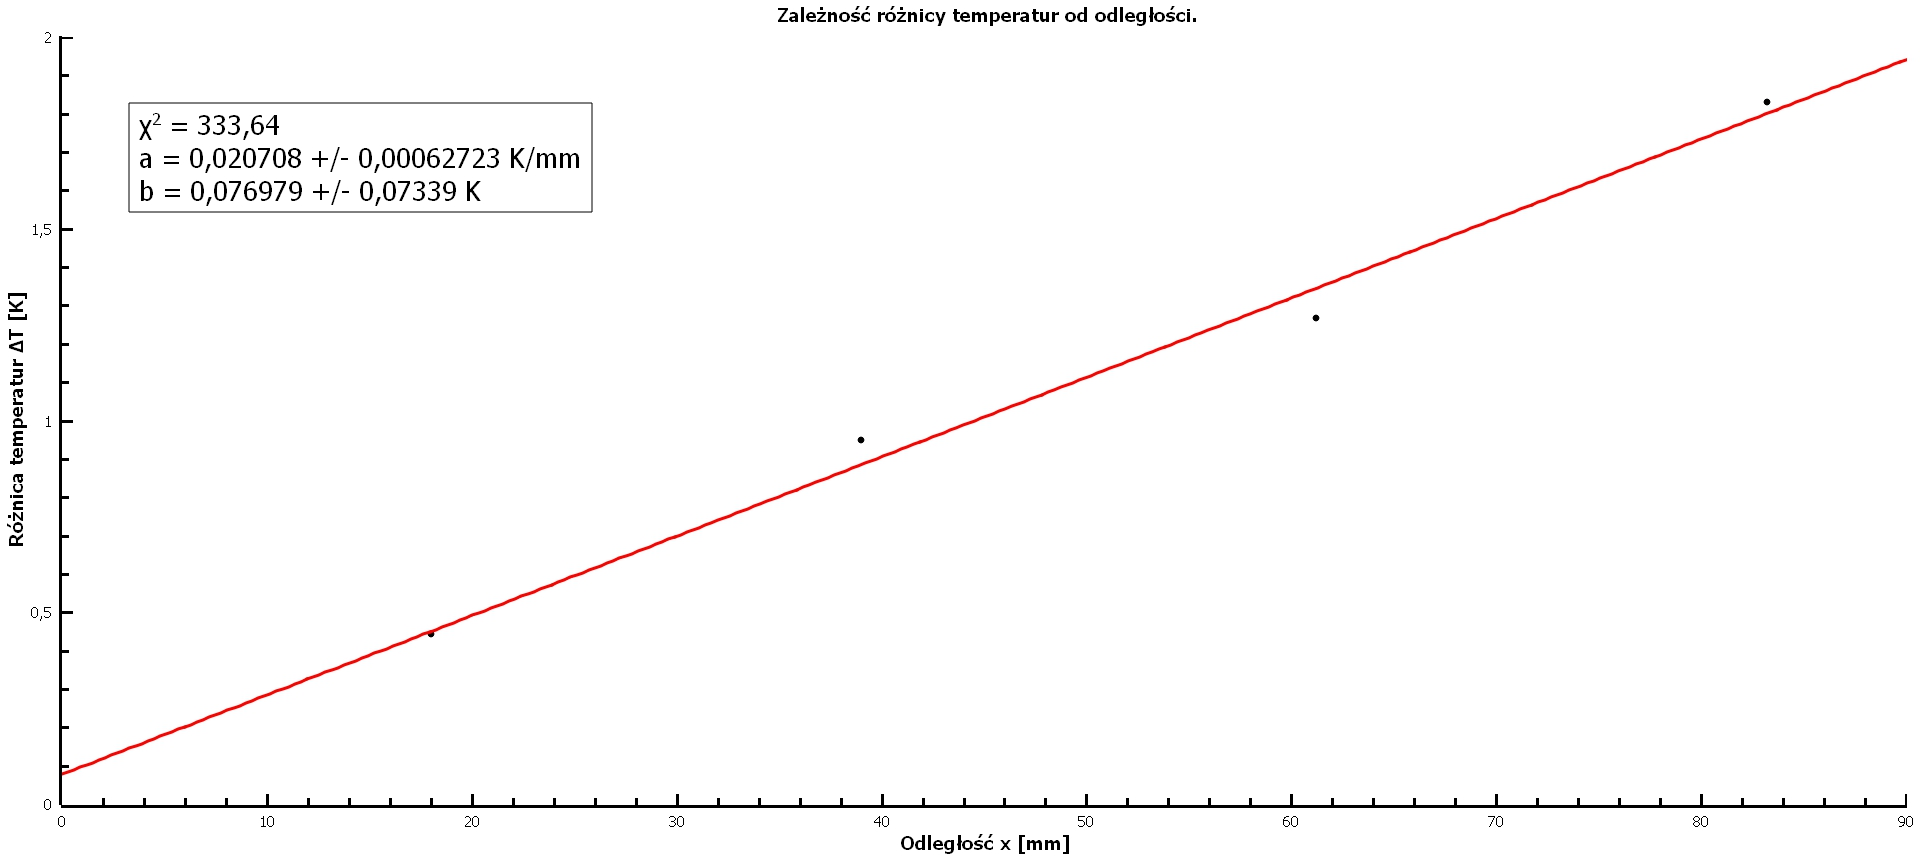
\includegraphics[width=15cm]{rap8rys7} 
\centering
\caption{$\Delta T (x)$: pomiar 1.}
\end{figure}

\begin{figure}[h!]
\centering
\begin{minipage}{0.5\textwidth}
  \centering
  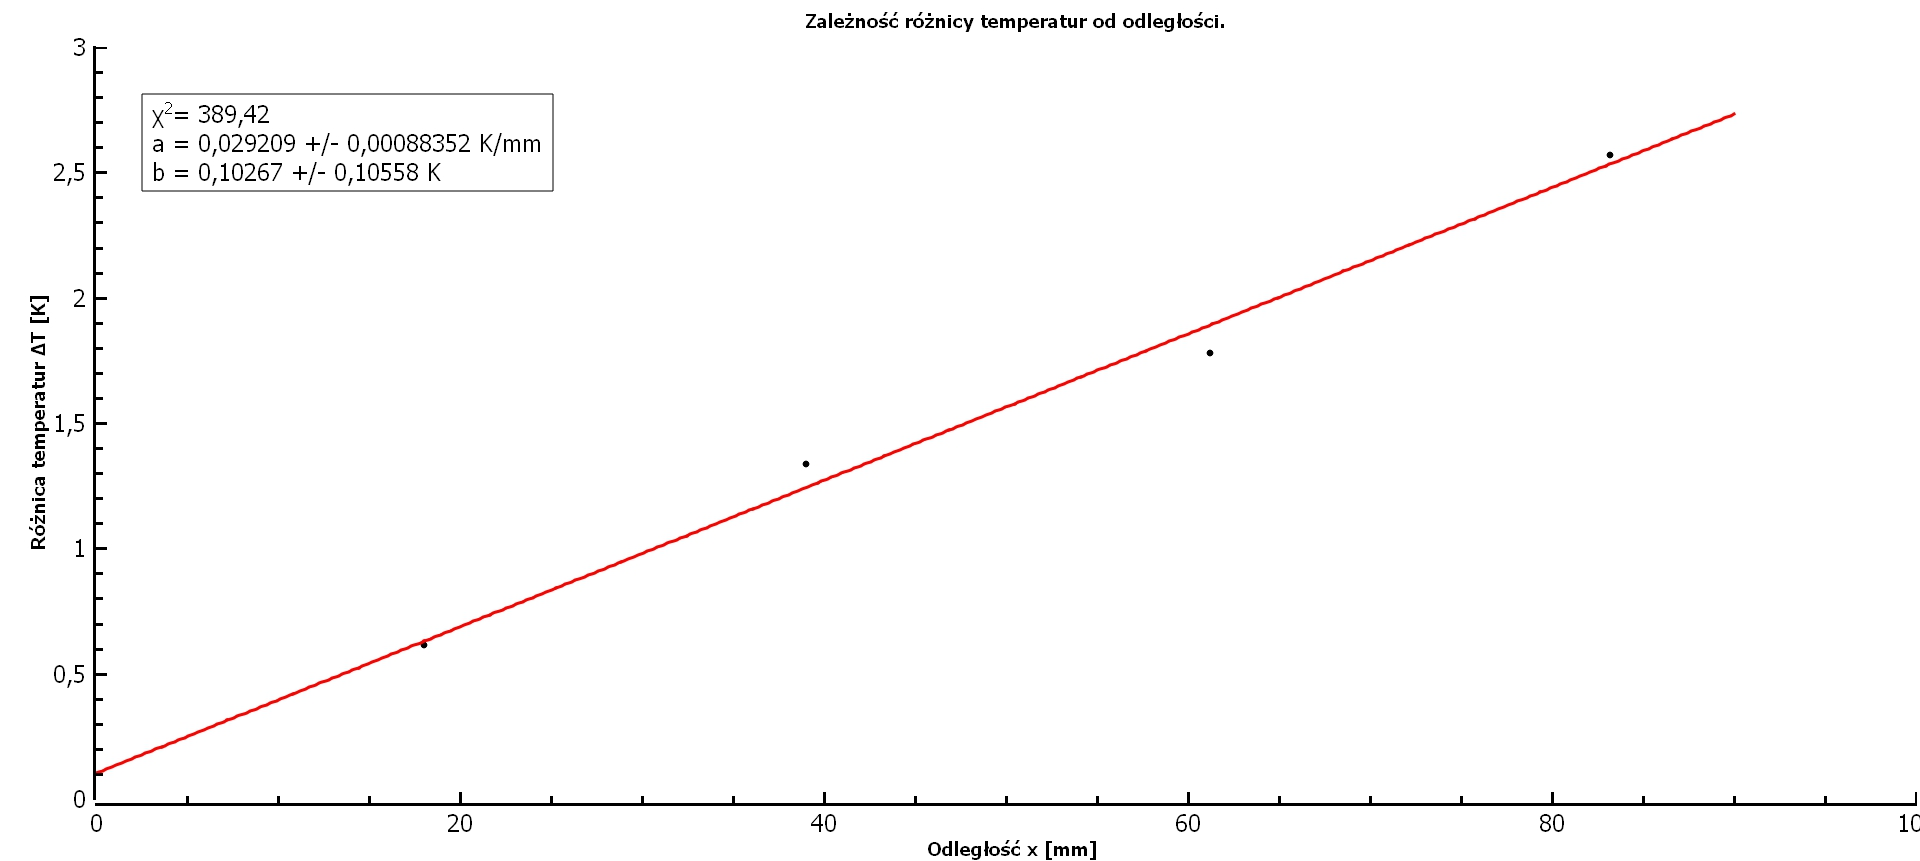
\includegraphics[width=8cm, height=5cm ]{rap8rys8} 
\caption{$\Delta T (x)$: pomiar 2.}
\end{minipage}%
\begin{minipage}{0.5\textwidth}
  \centering
  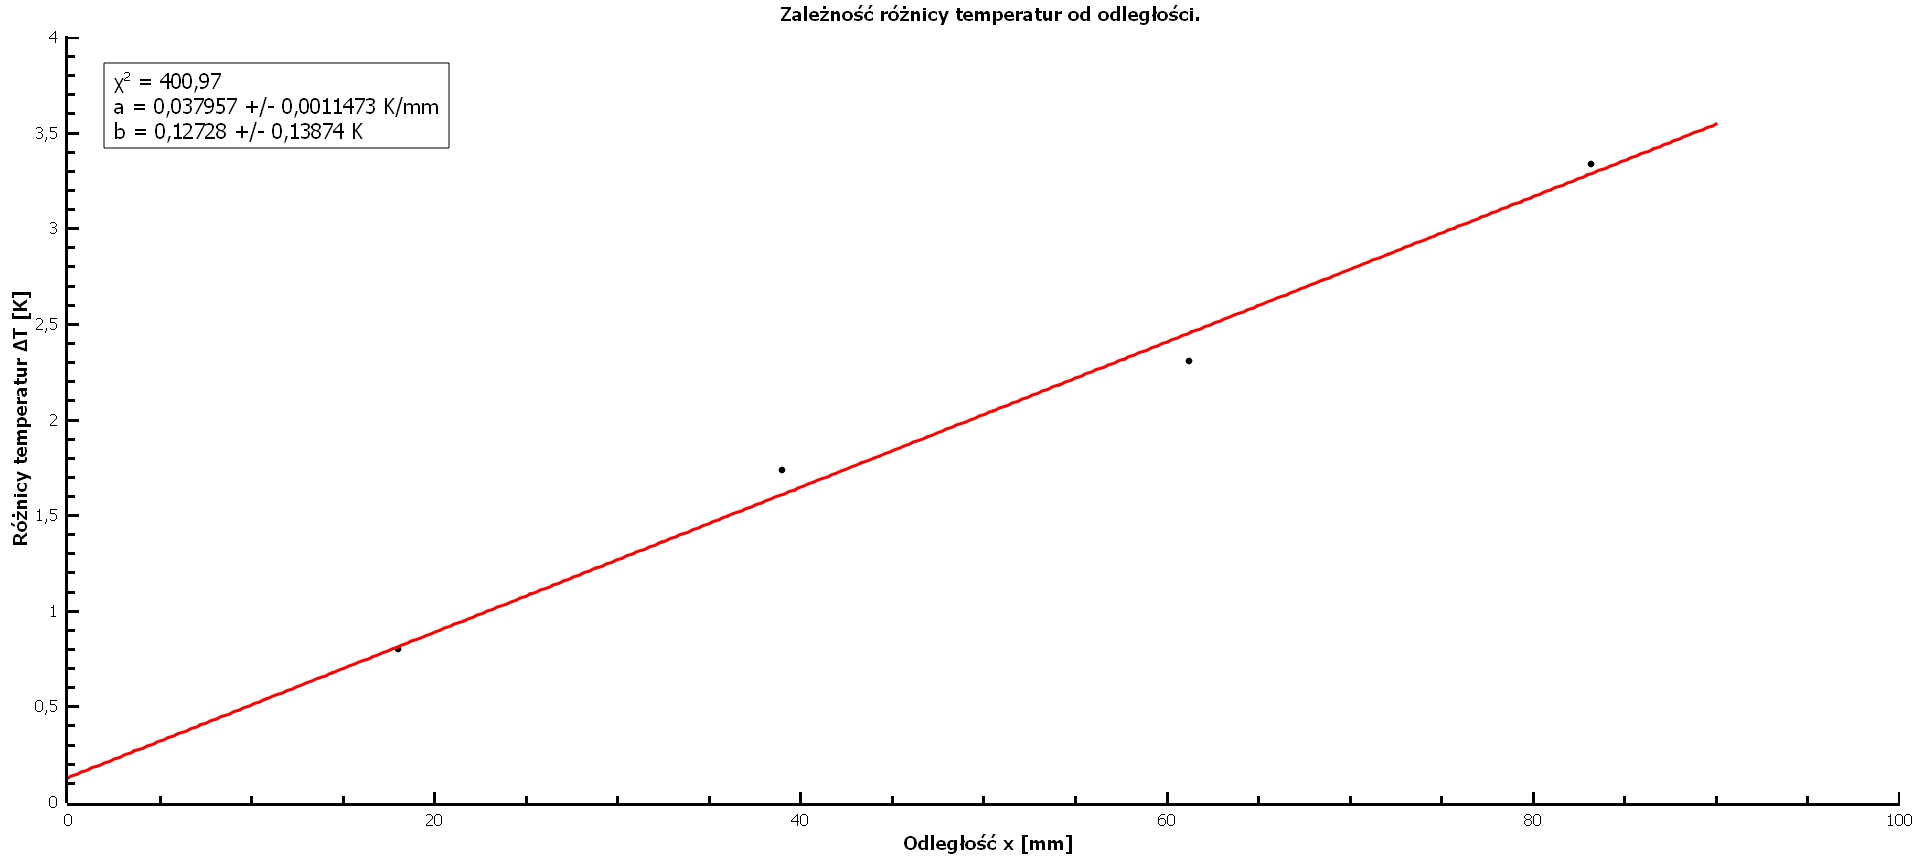
\includegraphics[width=8cm, height=5cm ]{rap8rys9} 
\caption{$\Delta T (x)$: pomiar 3.}
\end{minipage}
\end{figure}

\begin{figure}[h!]
\centering
\begin{minipage}{0.5\textwidth}
  \centering
  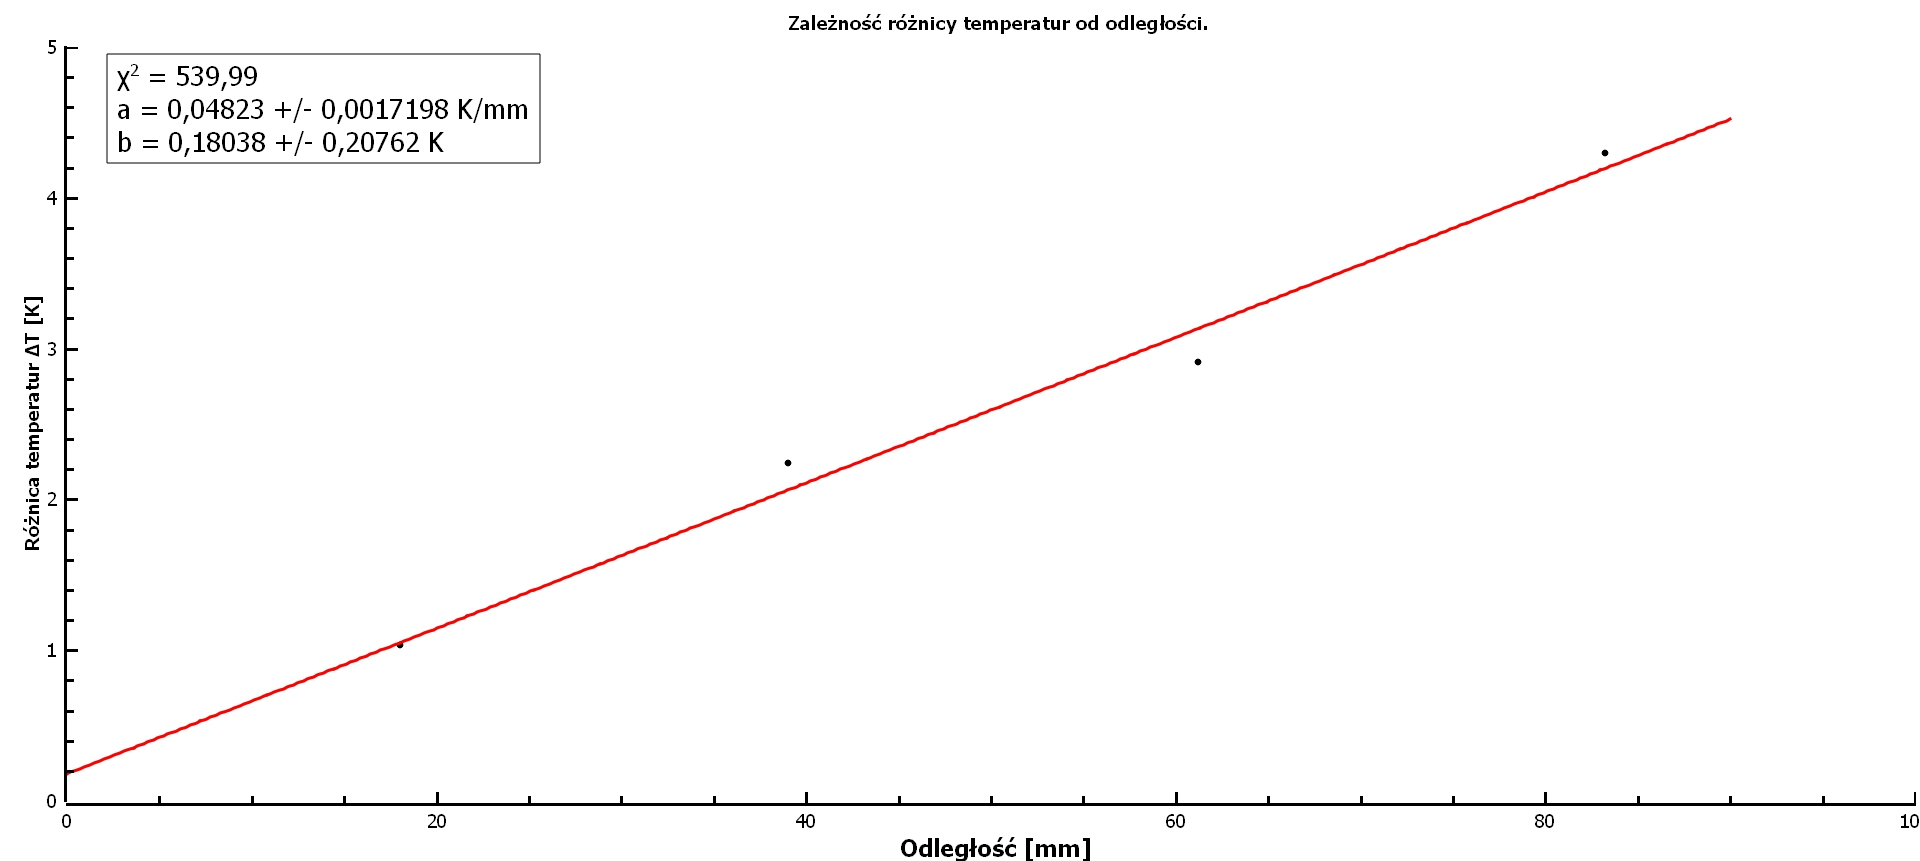
\includegraphics[width=8cm, height=5cm ]{rap8rys10} 
\caption{$\Delta T (x)$: pomiar 4.}
\end{minipage}%
\begin{minipage}{0.5\textwidth}
  \centering
  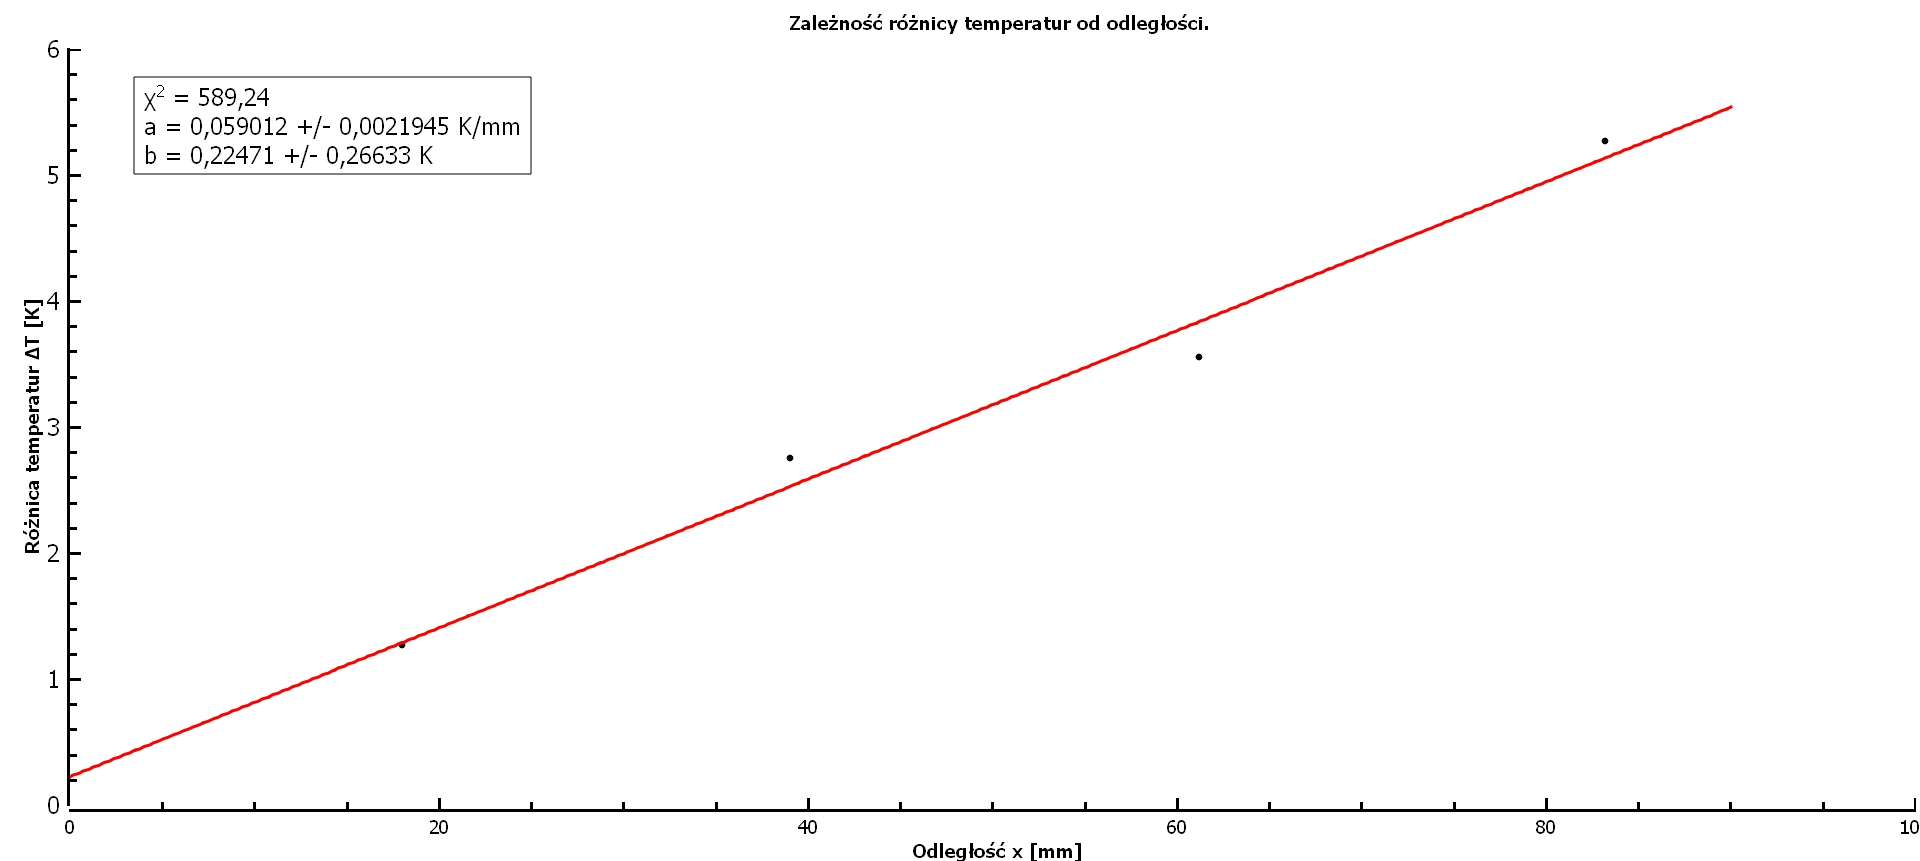
\includegraphics[width=8cm, height=5cm ]{rap8rys11} 
\caption{$\Delta T (x)$: pomiar 5.}
\end{minipage}
\end{figure}

Mimo to postanowiono kontynuować analizę danych. Otrzymane współczynniki kierunkowe przyporządkowano do odpowiednich mocy grzałki. Moc grzałki $P=UI$ obliczono, korzystając z danych z Tabeli 1, a niepewność tej mocy wyznaczono korzystając z Równania (6). Otrzymano:
\begin{equation}
 u_{P}=P \sqrt{\dfrac{u_{U}^2}{U^2}+\dfrac{u_{I}^2}{I^2}}
 \end{equation}
 Dodatkowo uwzględniono, że nie cało mac grzałki jest przekazywana prętowi. Postanowiono przyjąć, iż sprawność grzałki wynosi $\eta=0,49\pm0,05$. 
 Niepewność mocy $\eta P$ wynosi, na mocy Równania (6):
 \begin{equation}
 u_{\eta P}=\eta P \sqrt{\dfrac{u_{P}^2}{P^2}+\dfrac{u_{\eta}^2}{\eta^2}}
 \end{equation}
Tabela 7 przedstawia wartości $\eta P$ wraz z niepewnościami oraz wartości współczynników kierunkowych wraz z ich niepewnościami.
\begin{table}[h!]
\centering
\caption{Wartości mocy i gradientu}
\begin{tabular}{|c|c|c|c|}
\hline
Współczynnik a [K/mm] & $\eta P$ [W] & $u_{a}$ [K/mm] & $u_{\eta P}$ [W] \\ \hline
0,021                 & 0,206        & 0,00063        & 0,0212           \\ \hline
0,030                 & 0,280        & 0,00088        & 0,0288           \\ \hline
0,038                 & 0,368        & 0,00115        & 0,0378           \\ \hline
0,048                 & 0,466        & 0,00172        & 0,048            \\ \hline
\end{tabular}
\end{table}
Zgodnie z Równaniem (1) wartości z Tabeli 8 podlegają następującemu rozkładowi:
\begin{equation}
\eta P+P_{0}=\lambda S a,
\end{equation}
gdzie $P_{0}$ jest mocą dostarczaną z otoczenia. Na podstawie danych z Tabeli 8 stworzono wykres wraz z krzywa najlepszego dopasowania, przedstawiony na Rysunku 12.

\begin{figure}[h!]
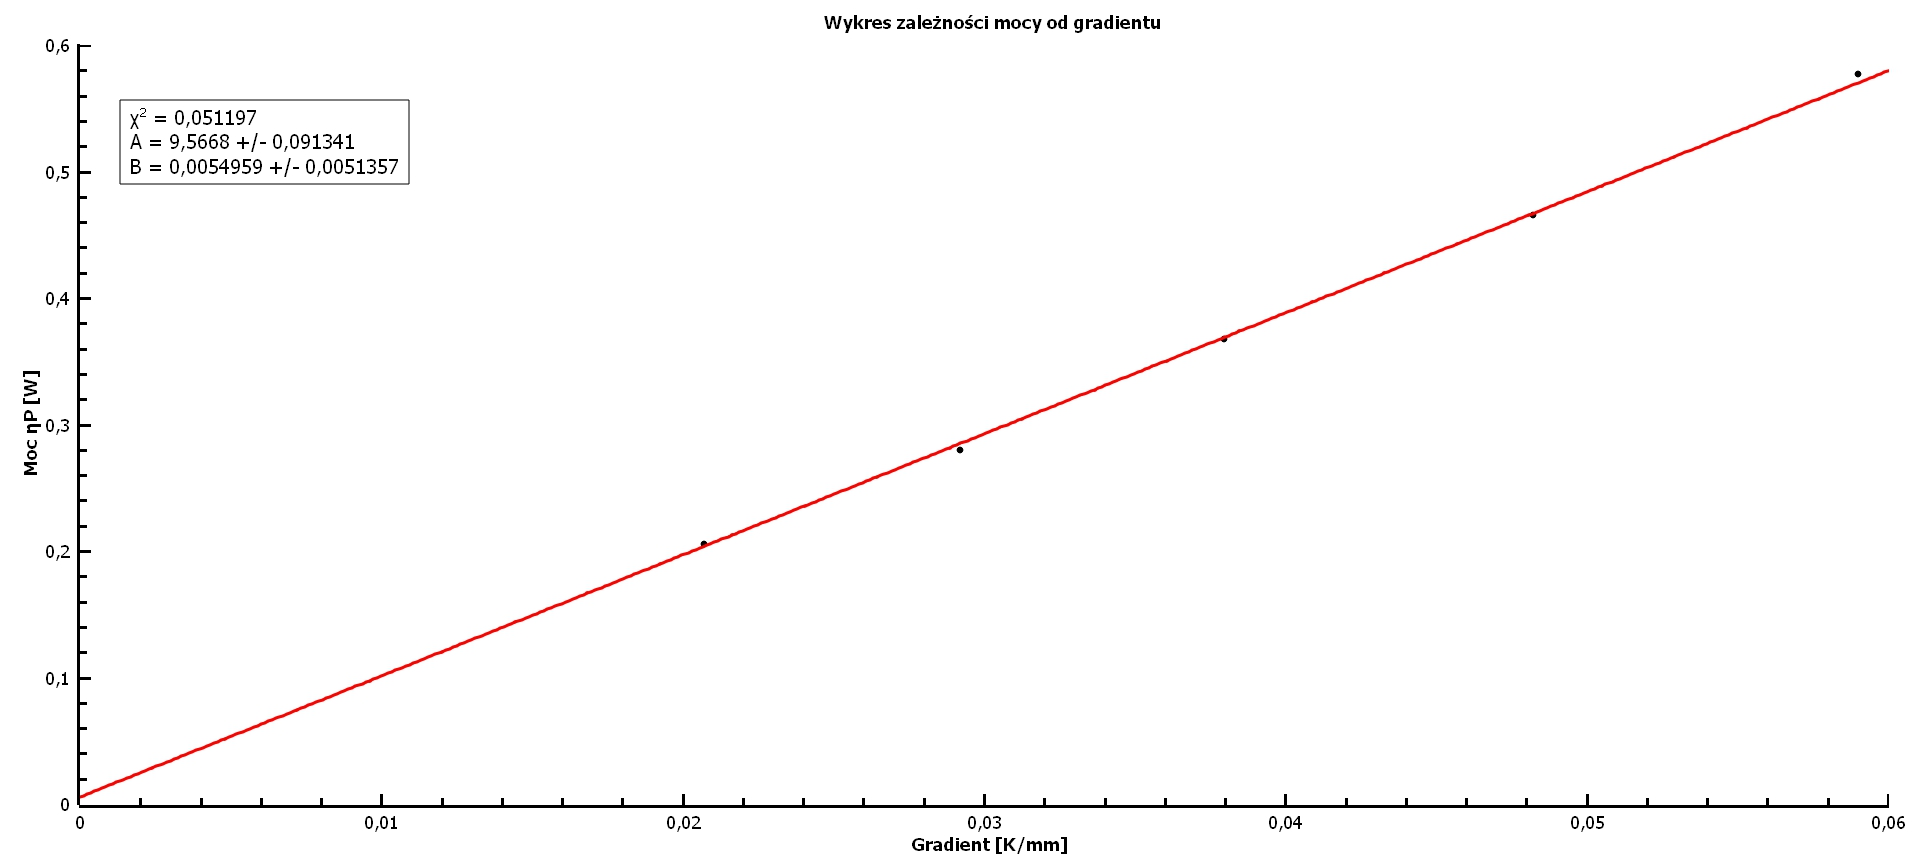
\includegraphics[width=15cm]{rap8rys12} 
\centering
\caption{$\eta P (a)$}
\end{figure}
Obliczone współczynniki wynoszą: $A=\lambda S$, $B=-P_{0}$. Zgodnie z oczekiwaniami, wymiana ciepła z otoczeniem jest niewielka. 
 
Korzystając z wartości współczynnika $A$ oraz $S=(\pi D^2)/4$ obliczono wartości $\lambda=344,02$ W/mK. Niepewność tej wielkości obliczono ponownie korzystając z Równania (6) otrzymując:
\begin{equation}
 u_{\lambda}=\lambda \sqrt{\dfrac{u_{A}^2}{A^2}+\dfrac{u_{S}^2}{S^2}}
 \end{equation}
 Po podstawieniu danych liczbowych otrzymano ostatecznie $\lambda=344\pm12$ w/mK.
 
  Postanowiono porównać tę wartość z wartością tablicową wynoszącą 385 W/mK \cite{c1}. Posłużono się w tym celu testem 3$\sigma$, który polega na sprawdzeniu, czy różnica między wartością teoretyczną a eksperymentalną jest mniejsza od trzykrotności niepewności tej różnicy. W tym przypadku potraktowano wartość tablicową jako znaną dokładnie. Różnica wielkości wynosi 40,98 W/mK a $3u_{\lambda}=34,55$ W/mK. Jak się okazuje wyznaczona wartość nie jest zgodna z wartością tablicową. 

\begin{center}
\textbf{\subsection*{DYSKUSJA WYNIKÓW I WNIOSKI}}
\end{center} 
Otrzymany wynik nie jest zgodny z wartością wzorcową pomimo starannie przeprowadzonych pomiarów. Pewną wskazówką w analizie błędów jest dopasowywanie krzywej zależności temperatury od odległości. Żadna z tych krzywych nie przeszłą testu $\chi^2$ więc prawdopodobnie istnieje jakiś błąd w pomiarach lub dopasowywaniu krzywych do Równania (5), który choć początkowo niewidoczny, narastał w trakcie analizy i przechodzeniu przez kolejne jej kroki, by na samym końcu jego wpływ był znaczący. Dodatkowo warto byłoby powtórzyć pomiar z wykorzystaniem innego sprzętu, by wykluczyć możliwość wad w układzie doświadczalnym.

\begin{center}
\begin{thebibliography}{9}

\bibitem{tay1}
 J. R. Taylor,
 \emph{Wstęp do analizy błędu pomiarowego},
 PWN, Warszawa, 1995, s. 175.
 
 \bibitem{c1}
 Young, Hugh D.,
 \emph{University Physics},
 Addison-Wesley Pub. Co., 1992, Table 15-5.
 \end{thebibliography}

\end{center}


\end{document}